\documentclass[11pt]{amsart}
\usepackage{geometry}                % See geometry.pdf to learn the layout options. There are lots.
\geometry{letterpaper}                   % ... or a4paper or a5paper or ... 
%\geometry{landscape}                % Activate for for rotated page geometry
%\usepackage[parfill]{parskip}    % Activate to begin paragraphs with an empty line rather than an indent
\usepackage{graphicx}
\usepackage{amssymb}
\usepackage{epstopdf}
\DeclareGraphicsRule{.tif}{png}{.png}{`convert #1 `dirname #1`/`basename #1 .tif`.png}

\title{GPU Acceleration for t-SNE Maps}
\author{Jackson Walters}
%\date{}                                           % Activate to display a given date or no date

\begin{document}
\maketitle
%\section{}
%\subsection{}

Using Google Colab, I obtained access to a NVIDIA Tesla K80 with 12GB of VRAM for use on a trial basis. With this hardware, I was able to train models using cuML\footnote{https://github.com/rapidsai/cuml}, a GPU accelerated library including t-SNE. The data includes at least seven columns which are `diagnostic', which are: \\

\begin{itemize}
  \item TRAUSTREFLG=Trauma- and stressor-related disorders
  \item ANXIETYFLG=Anxiety disorders
  \item ADHDFLG=Attention deficit/hyperactivity disorder (ADHD)
  \item BIPOLARFLG=Bipolar disorders
  \item DEPRESSFLG=Depressive disorders
  \item SCHIZOFLG=Schizophrenia or other psychotic disorders
  \item PERSONFLG=Personality disorders
\end{itemize}

\vspace{5mm}

These are binary, 0/1 indicators of a diagnosed disorder. Since there are seven categories, this yields 128 discrete categories. This is too many for visualization purposes, so we cut them down by choosing one for 'no-disorder' (all zeros), one for 'single disorder' (one 1 and the rest zeros), and 'multi-disorder' (more than one 1). This yields nine categories. The t-SNE with perplexity around 10 reveals clear clusters:

\begin{figure}[h]
\caption{num-data-points=10,000. Mental health diagnostic data mapped to 2d using t-SNE. Note there is no symptom or life-factor data in this dataset yet. There is one 'no-disorder' category, seven unique disorder categories, and one multi-disorder category. We observe eight clusters, with the multi-disorder categories appearing scattered.}
\centering
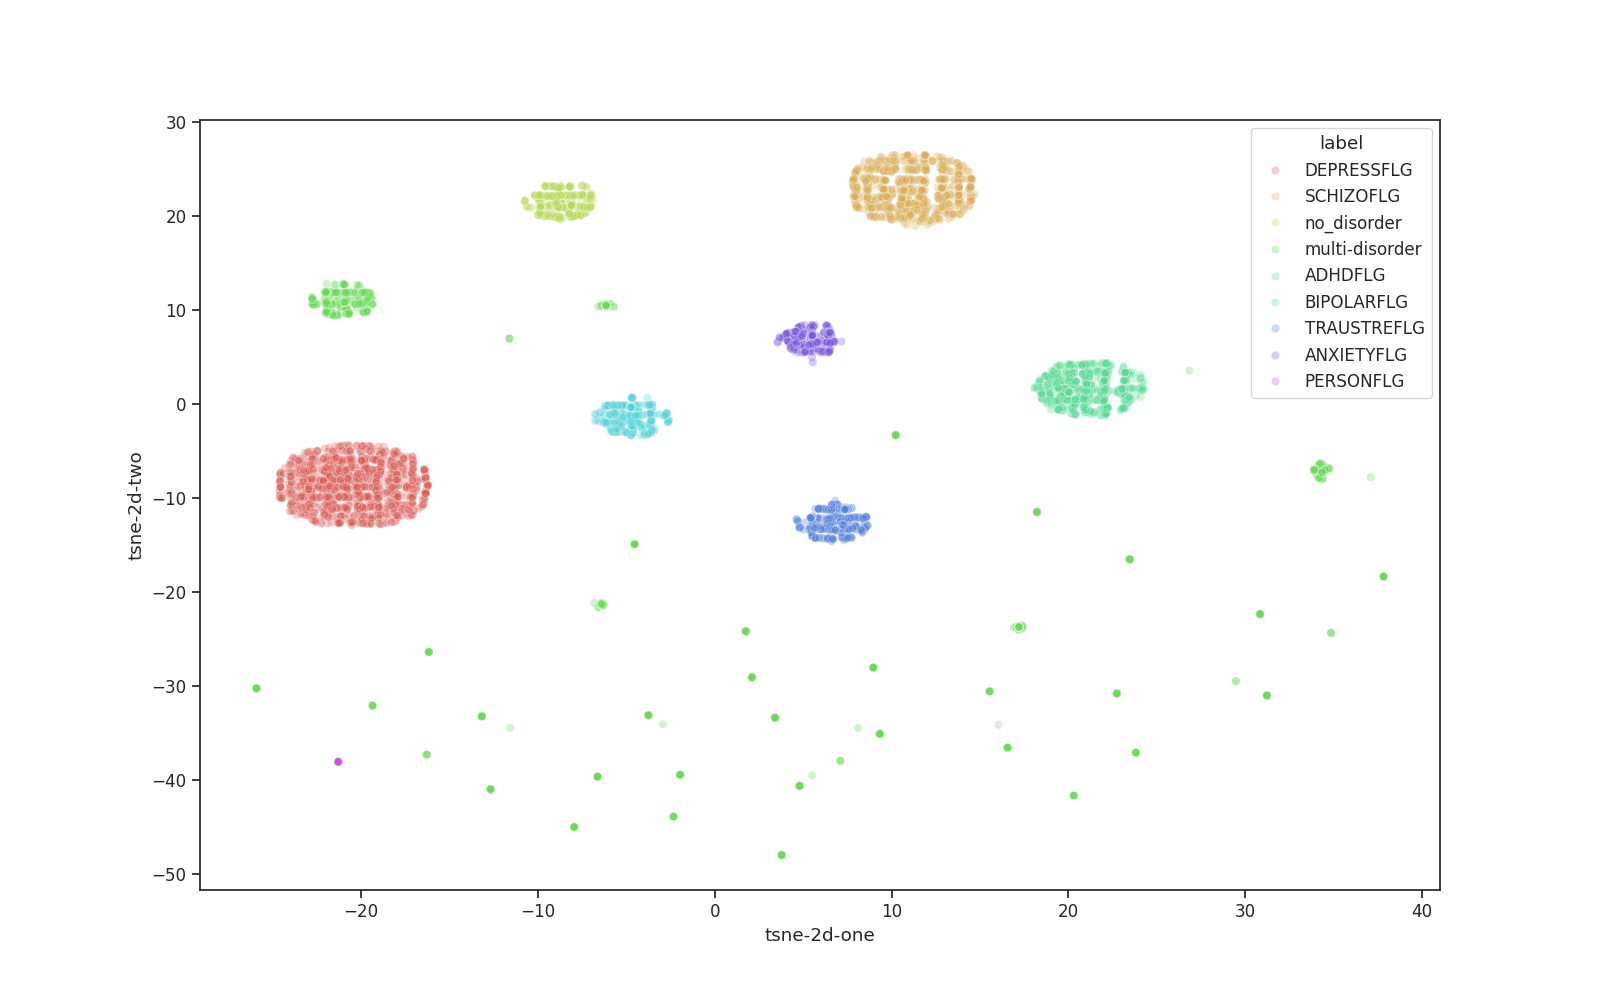
\includegraphics[width=1.0\textwidth]{tsne_plot_mental-health_client-level-data_perplexity=10_num-points=10_000_labeled}
\end{figure}




\end{document}  